\subsection{Среда Ant}

В качестве полигона для исследования возможностей нейроэволюции была выбрана среда непрерывного управления Ant-v4 из библиотеки Gymnasium. Данная среда представляет собой физическую симуляцию на базе движка MuJoCo, описанную в \cite{mujoco}, для четырехногого агента («муравья»), цель которого -- максимально быстро и эффективно продвигаться вперед (по оси X), сохраняя при этом баланс и минимизируя затраты энергии на лишние движения.

\begin{figure}[h!]
  \centering
  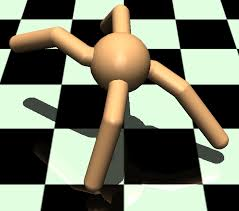
\includegraphics[width=0.6\textwidth]{./images/ant.png}
  \caption{Схематическое изображение агента в среде Ant-v4.}
  \label{fig:ant}
\end{figure}

\subsubsection{Пространство состояний и действий}

Сложность среды обусловлена физическими параметрами модели:

\begin{itemize}

  \item Пространство состояний (27 параметров): включает в себя данные о положении корпуса в пространстве, углы поворота всех восьми сочленений, а также векторы их линейных и угловых скоростей. Такой объем данных необходим нейросети для понимания текущей позы робота и инерции его частей.

  \item Пространство действий (8 параметров): агент управляет крутящими моментами, прикладываемыми к каждому из восьми суставов. Действия являются непрерывными и лежат в диапазоне $[-1, 1]$.
\end{itemize}

\subsubsection{Функция награды и условия завершения}

Функция приспособленности в данном эксперименте базируется на стандартной системе вознаграждений Ant-v4, которая включает:

\begin{enumerate}

  \item Reward for moving forward: поощрение за продвижение вдоль оси X.

  \item Healthy reward: фиксированный бонус за каждый шаг, пока робот остается «здоров» (не перевернулся и не вышел за пределы допустимых углов).

  \item Control cost: штраф за слишком резкие или энергозатратные движения, что стимулирует агента к плавной и естественной походке.

\end{enumerate}

Для оптимизации процесса эволюции была внедрена эвристика «жесткого таймера». Если в течение 50 шагов симуляции агент не продвигается вперед более чем на 0.05 метра, эпизод прерывается досрочно. Это позволяет алгоритму быстрее переходить к оценке следующей особи, не тратя время на агентов, которые застряли или совершают хаотичные движения на месте. Окончательная оценка генома вычисляется как среднее арифметическое результатов трех независимых эпизодов.

\subsubsection{Конфигурация алгоритма NEAT для среды Ant-v4}


\href{https://github.com/Isn0v/neat-training/blob/master/environments/ant/neat.cfg}{Настройка}\footnote{\url{https://github.com/Isn0v/neat-training/blob/master/environments/ant/neat.cfg}} алгоритма NEAT для среды Ant-v4 оказалась непростой задачей. Главная сложность заключалась в высокой размерности пространства действий: малейшие хаотичные скачки в топологии растущей сети могли легко разрушить только начавший формироваться навык ходьбы агента. Чтобы взять этот процесс под контроль, мы разделили архитектуру решения на три обособленных блока: базовые архитектурные параметры, генетические механизмы и саму вычислительную инфраструктуру.

\paragraph{Архитектурные параметры и инициализация:}

Стартовую архитектуру нейросетей мы также сделали примитивной. Размерность слоев мы жестко привязали к физической модели «муравья»: сеть получила 27 сенсорных узлов на входе и 8 моторных на выходе.

Как и в предыдущих экспериментах, мы полностью отказались от использования скрытых нейронов на старте. Все сенсорные данные напрямую пробрасывались на выходы. Подобный подход давал эволюции возможность сперва отточить базовые линейные зависимости в управлении роботом, и лишь затем, по мере необходимости, выстраивать сложные нелинейные цепи.

Для выходных сигналов идеально подошел гиперболический тангенс, потому что он совпадает с требованиями физического движка MuJoCo к управляющим импульсам. При этом классическое суммирование входящих сигналов внутри узлов мы заменили на усреднение.

\paragraph{Генетические операторы и мутации:}

\begin{itemize}

  \item Генетические операторы: Для обеспечения баланса между эксплуатацией текущих решений и исследованием новых топологий были установлены следующие коэффициенты:

  \item Мутация весов и смещений: используется гауссово распределение со средним значением 0.0 и стандартным отклонением 0.1. Максимальные и минимальные значения весов ограничены диапазоном $[-3.0, 3.0]$ для предотвращения «взрыва» активаций в глубоких слоях эволюционирующей сети.

  \item Структурные мутации: вероятность добавления новой связи (conn\_add\_prob) составляет 0.3, а добавления нового узла (node\_add\_prob) -- 0.1. При этом вероятности удаления компонентов (conn\_delete\_prob, node\_delete\_prob) установлены в 0, что гарантирует сохранение накопленной сложности топологии в рамках данного эксперимента. Данное решение было принято для ускорения сходимости, так как большинство полезных мутаций в Ant-v4 связано с добавлением новых связей, а не удалением существующих.

\end{itemize}

\paragraph{Видообразование и репродукция:}

Порог генетической совместимости был зафиксирован на отметке 1.2. На практике это позволило аккуратно дробить обширную популяцию из 500 особей на изолированные, устойчивые группы с похожими топологиями сетей. Внутри каждого сформированного вида гарантированно выживала только одна лучшая особь, тогда как для популяции в целом этот лимит составлял 5 агентов, набравших наибольший результат приспособленности. Право участвовать в кроссинговере и передавать свои гены следующему поколению получали лишь 20\% наиболее результативных агентов.

\paragraph{Инфраструктура обучения и отказоустойчивость:}

Перейдем к технической реализация, находящейся в файле \href{https://github.com/Isn0v/neat-training/blob/master/environments/ant/model.py}{model.py}\footnote{\url{https://github.com/Isn0v/neat-training/blob/master/environments/ant/model.py}}.

Вычисления в среде Ant-v4 ресурсоемки, поэтому нам пришлось внедрить ряд решений для обеспечения стабильности экспериментов.  Во-первых, мы ушли от последовательного выполнения кода и распределили расчет приспособленности агентов на все доступные ядра процессора с помощью инструмента ParallelEvaluator. Такая параллелизация позволила радикально ускорить симуляцию, сократив время обработки одного поколения примерно в 4–8 раз в соответствии с количеством физических ядер устройства.  Во-вторых, мы учли тот факт, что эволюция многосуставного робота — это тяжелый процесс, который может длиться от нескольких часов до нескольких дней. В таких условиях очень важной оказалась отказоустойчивость. Мы настроили систему чекпоинтов и теперь алгоритм автоматически делает полный срез популяции и сохраняет весь накопленный прогресс каждые 25 поколений. Это надежно страховало нас от потери результатов в случае любых системных сбоев или переполнения памяти. 